\section{}
\textbf{NOTE: } the values of $t_I=3$ has been used as $t_i=2$ leads to the infection dying out in around 20 days.


\begin{figure}[h!]
    \begin{center}
        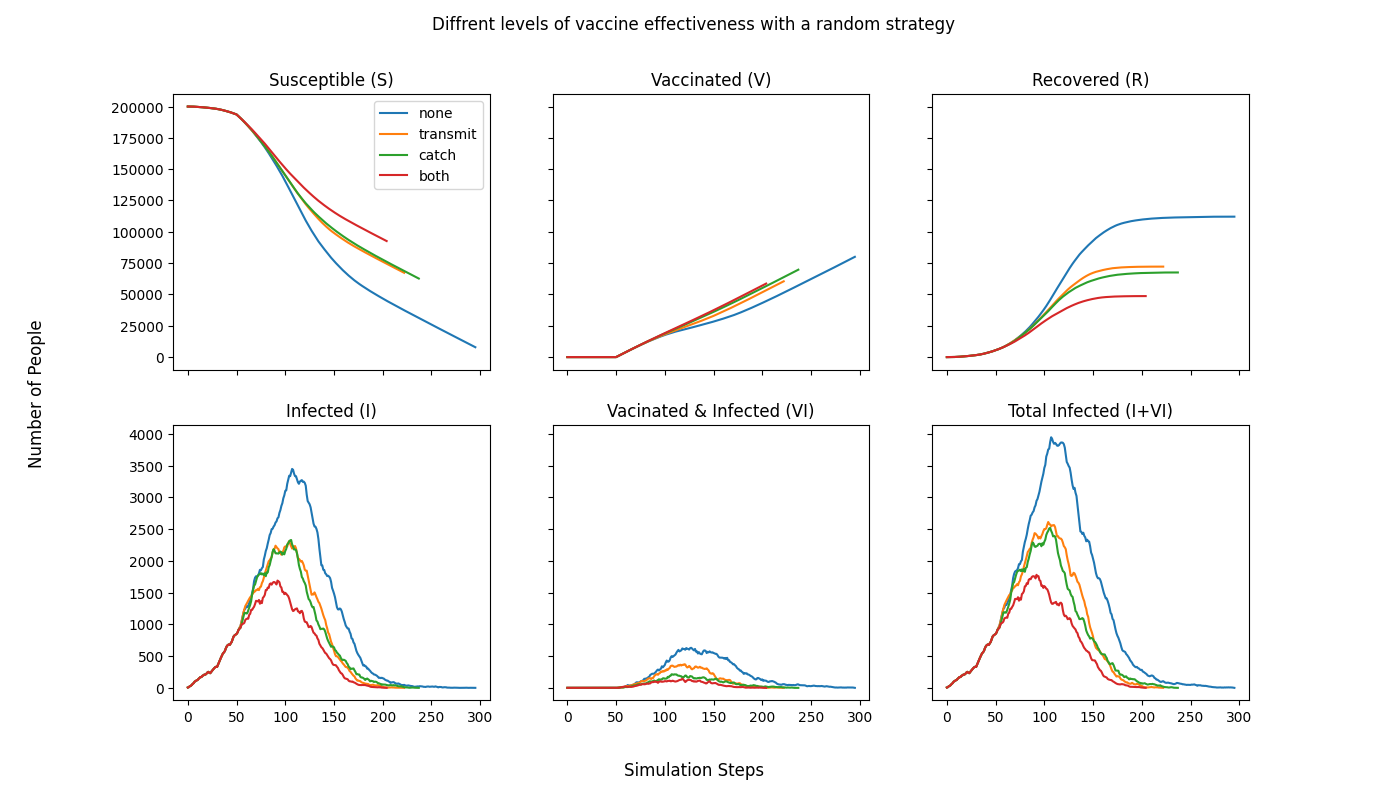
\includegraphics[width=1\textwidth]{Q5.png}
        \caption{Figure showing the how changing the the effectiveness of the vaccine effects the course of an outbreak. Blue - the vaccine has no effect. Yellow - the vaccine reduces transmission. Green - the vaccine reduces susceptibility. Red - the vaccine reduces transmission and susceptibility.} 
        \label{fig:q5}
    \end{center}
\end{figure}
We tested 4 different scenarios, where the vaccine: had no effect, reduces transmission, reduces susceptibility and reduces both transmission and susceptibility.
The probabilities used are normalized and listed below.
\begin{center}
\begin{tabular}{ccccc}
    &\multicolumn{4}{c}{Normalized probabilities}\\
    & P(I,S) & P(I, V) & P(VI, S) & P(VI, V)\\
    \hline
    No effect & 1 & 1& 1& 1 \\
    Transmission & 1 & 1& 0.5& 0.5 \\
    Susceptibility& 1 & 0.5& 1& 0.5 \\
    Both & 1 & 0.5 & 0.5 & 0.25 \\
\end{tabular}
\end{center}

We can see in Figure \ref{fig:q5} that an effective vaccine made a significant difference to the length of the outbreak.
When the vaccine was ineffective the outbreak ended on day 296.
However when the vaccine lowered transmission, lowered susceptibility and lowered both the outbreak ended on days 223, 238, 205 respectively.
Lowering both transmission and susceptibility unsurprisingly is the best in terms of stopping the outbreak.
And over the course of multiple repeats of the experiment lowering transmission and lowering susceptibility have an approximately equivalent effect.